This section explores how core composition performance depends on branch prediction, fetching mechanism, and data dependencies between blocks and how modifications to certain mechanisms can improve performance.
\vspace{-1em}
\subsection{Branch prediction}
\begin{figure}[t]
    \centering
    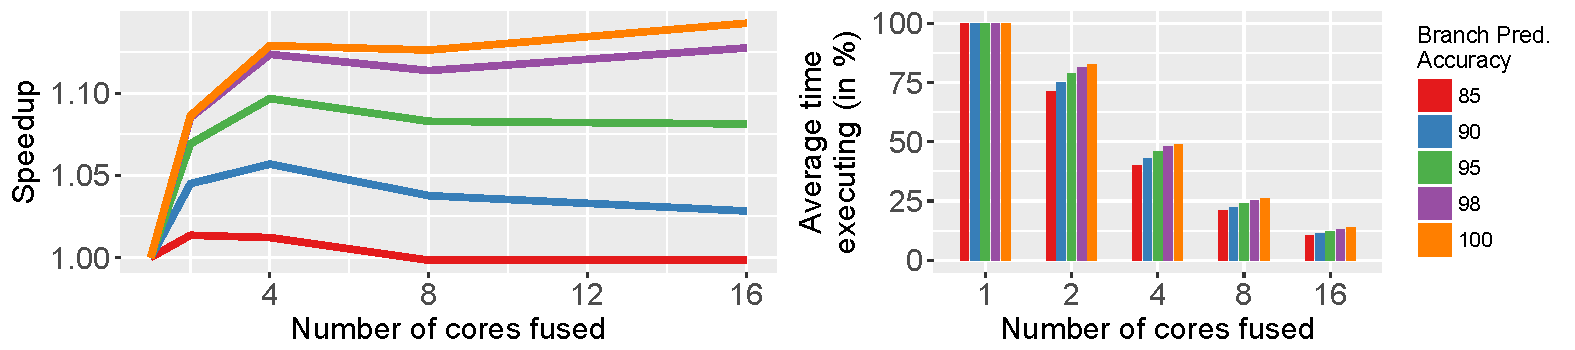
\includegraphics[width=1\textwidth]{chapter3/graphics/motiv_p1.pdf}
    \caption{Left: Speedup obtained when executing the MSER benchmark on different compositions and branch prediction accuracies.
	Right: Percentage of time (in cycles) cores in a composition execute instructions compared to the overall execution time. Higher is better for both.}
    \label{fig:mser_motiv}
    \centering
    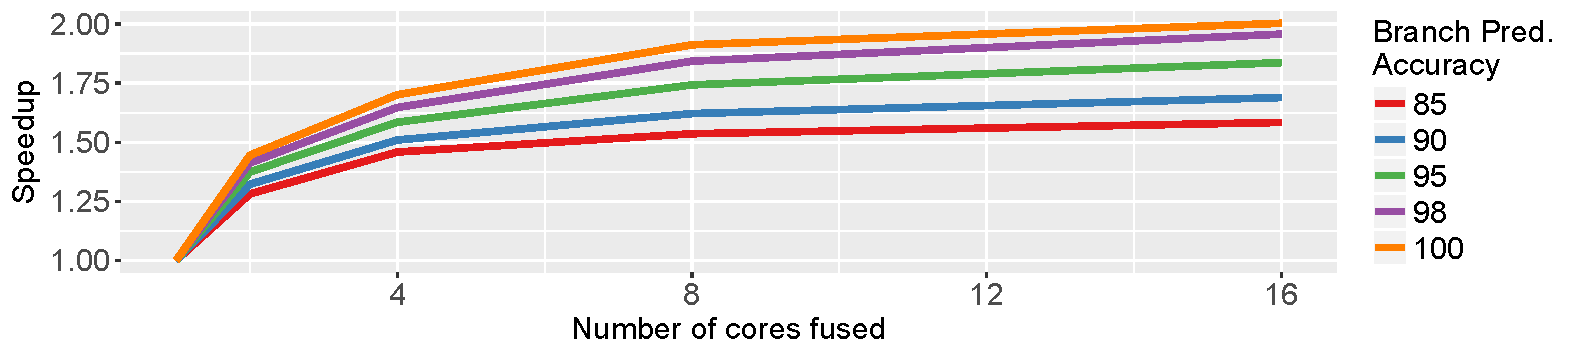
\includegraphics[width=1\textwidth]{chapter3/graphics/perfect_fetch_motiv2.pdf}
    \caption{Speedup obtained when executing the MSER benchmark with different core composition with an oracle fetching scheme and perfect branch prediction. Higher is better. }
    \label{fig:motivation_fetch}
	\vspace{1em}
\end{figure}
Chapter~\ref{chp:cases} section~\ref{sec:lim_study} highlighted the importance of branch prediction accuracy when fusing a high number of cores.
To maximise utilisation, a core can have multiple blocks in its instruction window.
In this thesis, the instruction window is segmented into four lanes, each of which can hold a block of up to 32 instructions.
If the program executing mainly has small blocks, then if it is running on a 16 core composition, the branch prediction accuracy needs to be as high as 98\% to ensure that the cores are fetching blocks on the correct execution path (see Chapter~\ref{chp:cases} section~\ref{sec:lim_study}).

In Chapter~\ref{chp:cases}, \bm{MSER} had a low branch prediction accuracy of 85\%, leading to a performance improvement of only 1\% on a 2 core composition.
To see how difference accuracies affect performance, a branch predictor that can predict at different accuracy levels is used.
The left hand side of Figure~\ref{fig:mser_motiv} shows the speedup obtained when executing the SD-VBS benchmark \bm{MSER} on core compositions of size 2, 4, 8, 16 with different branch prediction accuracies on the cycle-accurate simulator.
The speedup is obtained by comparing the performance to a single core.
As the figure shows, increasing the accuracy to 100\% leads to a performance increase of 1.15x on a 16 core composition.


\subsection{Fetching mechanism}
The reason performance does not improve much is due to the fact that \bm{MSER} features small blocks.
Currently, when cores are composed, they fetch blocks in a serial fashion, as defined in Chapter~\ref{chp:Background} Section~\ref{chp:Background:sec:EDGE}.
As cores only submit fetch requests to other cores in the composition if they are full, this means that if a core is able to commit a block before being full, then it will never submit a fetch request to another core.
In this situation, cores in a composition may remain inactive during the execution of a program as they are not prompted to fetch blocks.
Throughout the rest of this chapter, this fetching scheme is referred to as Serial Fetch (SF).% (see Chapter~\ref{chp:Background} for more details).

To understand how the fetching scheme can affect performance, the simulator records the number of cycles each core is actively executing code.
The right hand side of figure~\ref{fig:mser_motiv} plots the average \textit{active cycles} of cores in a 1, 2, 4, 8 and 16 core composition, compared to the total execution time in cycles using SF, with different branch prediction accuracies.
The figure shows that increasing the size of a core composition when executing \bm{MSER} will reduce the average time a core is executing a block.
On a 16 core composition, each core is only actively executing a block 12.5\% of the time.
Cores are not being provisioned with blocks fast enough, thus, for a benchmark such as \bm{MSER}, the current fetching scheme leads to inefficient use of large compositions.
%This is why the performance improvements are only slight with perfect branch prediction.

To illustrate how modifying the fetching mechanism can improve performance of core composition, an oracle fetching mechanism (OF) is designed, in which cores can fetch in parallel and do not require any communication beyond receiving a prediction from another core.
Figure~\ref{fig:motivation_fetch} shows the speedup obtained by using the OF scheme on \bm{MSER} with different branch prediction accuracies and a baseline of a single core.
The figure shows that by modifying the fetching scheme a 16 core composition can potentially improve the performance of \bm{MSER} by 2x, compared to the 1.15x obtained when using the SF scheme.

\subsection{Data dependencies between blocks}

In the EDGE architecture, physical registers are used for inter-block communication.
For example, the code found in Listing~\ref{lst:mser_snipet} shows a loop found in the \bm{MSER} benchmark when the value of the variable \textit{nvisited}, which is used in both the header and loop body, will be passed from one block to another via a register read and write.

\lstset{
	backgroundcolor=\color{lbcolor},
	tabsize=2,
	rulecolor=,
	language=matlab,
        basicstyle=\tiny,
        upquote=true,
        aboveskip={1\baselineskip},
        columns=fixed,
        showstringspaces=false,
        extendedchars=true,
        breaklines=true,
        prebreak = \raisebox{0ex}[0ex][0ex]{\ensuremath{\hookleftarrow}},
        frame=single,
        showtabs=false,
        showspaces=false,
        showstringspaces=false,
        identifierstyle=\ttfamily,
        keywordstyle=\color[rgb]{0,0,1},
        commentstyle=\color[rgb]{0.133,0.545,0.133},
        stringstyle=\color[rgb]{0.627,0.126,0.941},
		numbers=left,
}

\begin{figure}[t]
\lstset{language=C,numbersep=4pt}
\begin{center}
\begin{lstlisting}
	while( nvisited-- ) {
				forest_pt [ sref(visited_pt,nvisited) ] .shortcut = nrindex ;
			}
\end{lstlisting}
\end{center}
\vspace{-2em}
\captionof{lstlisting}{Example of loop found in MSER.}
\label{lst:mser_snipet}
    \centering
    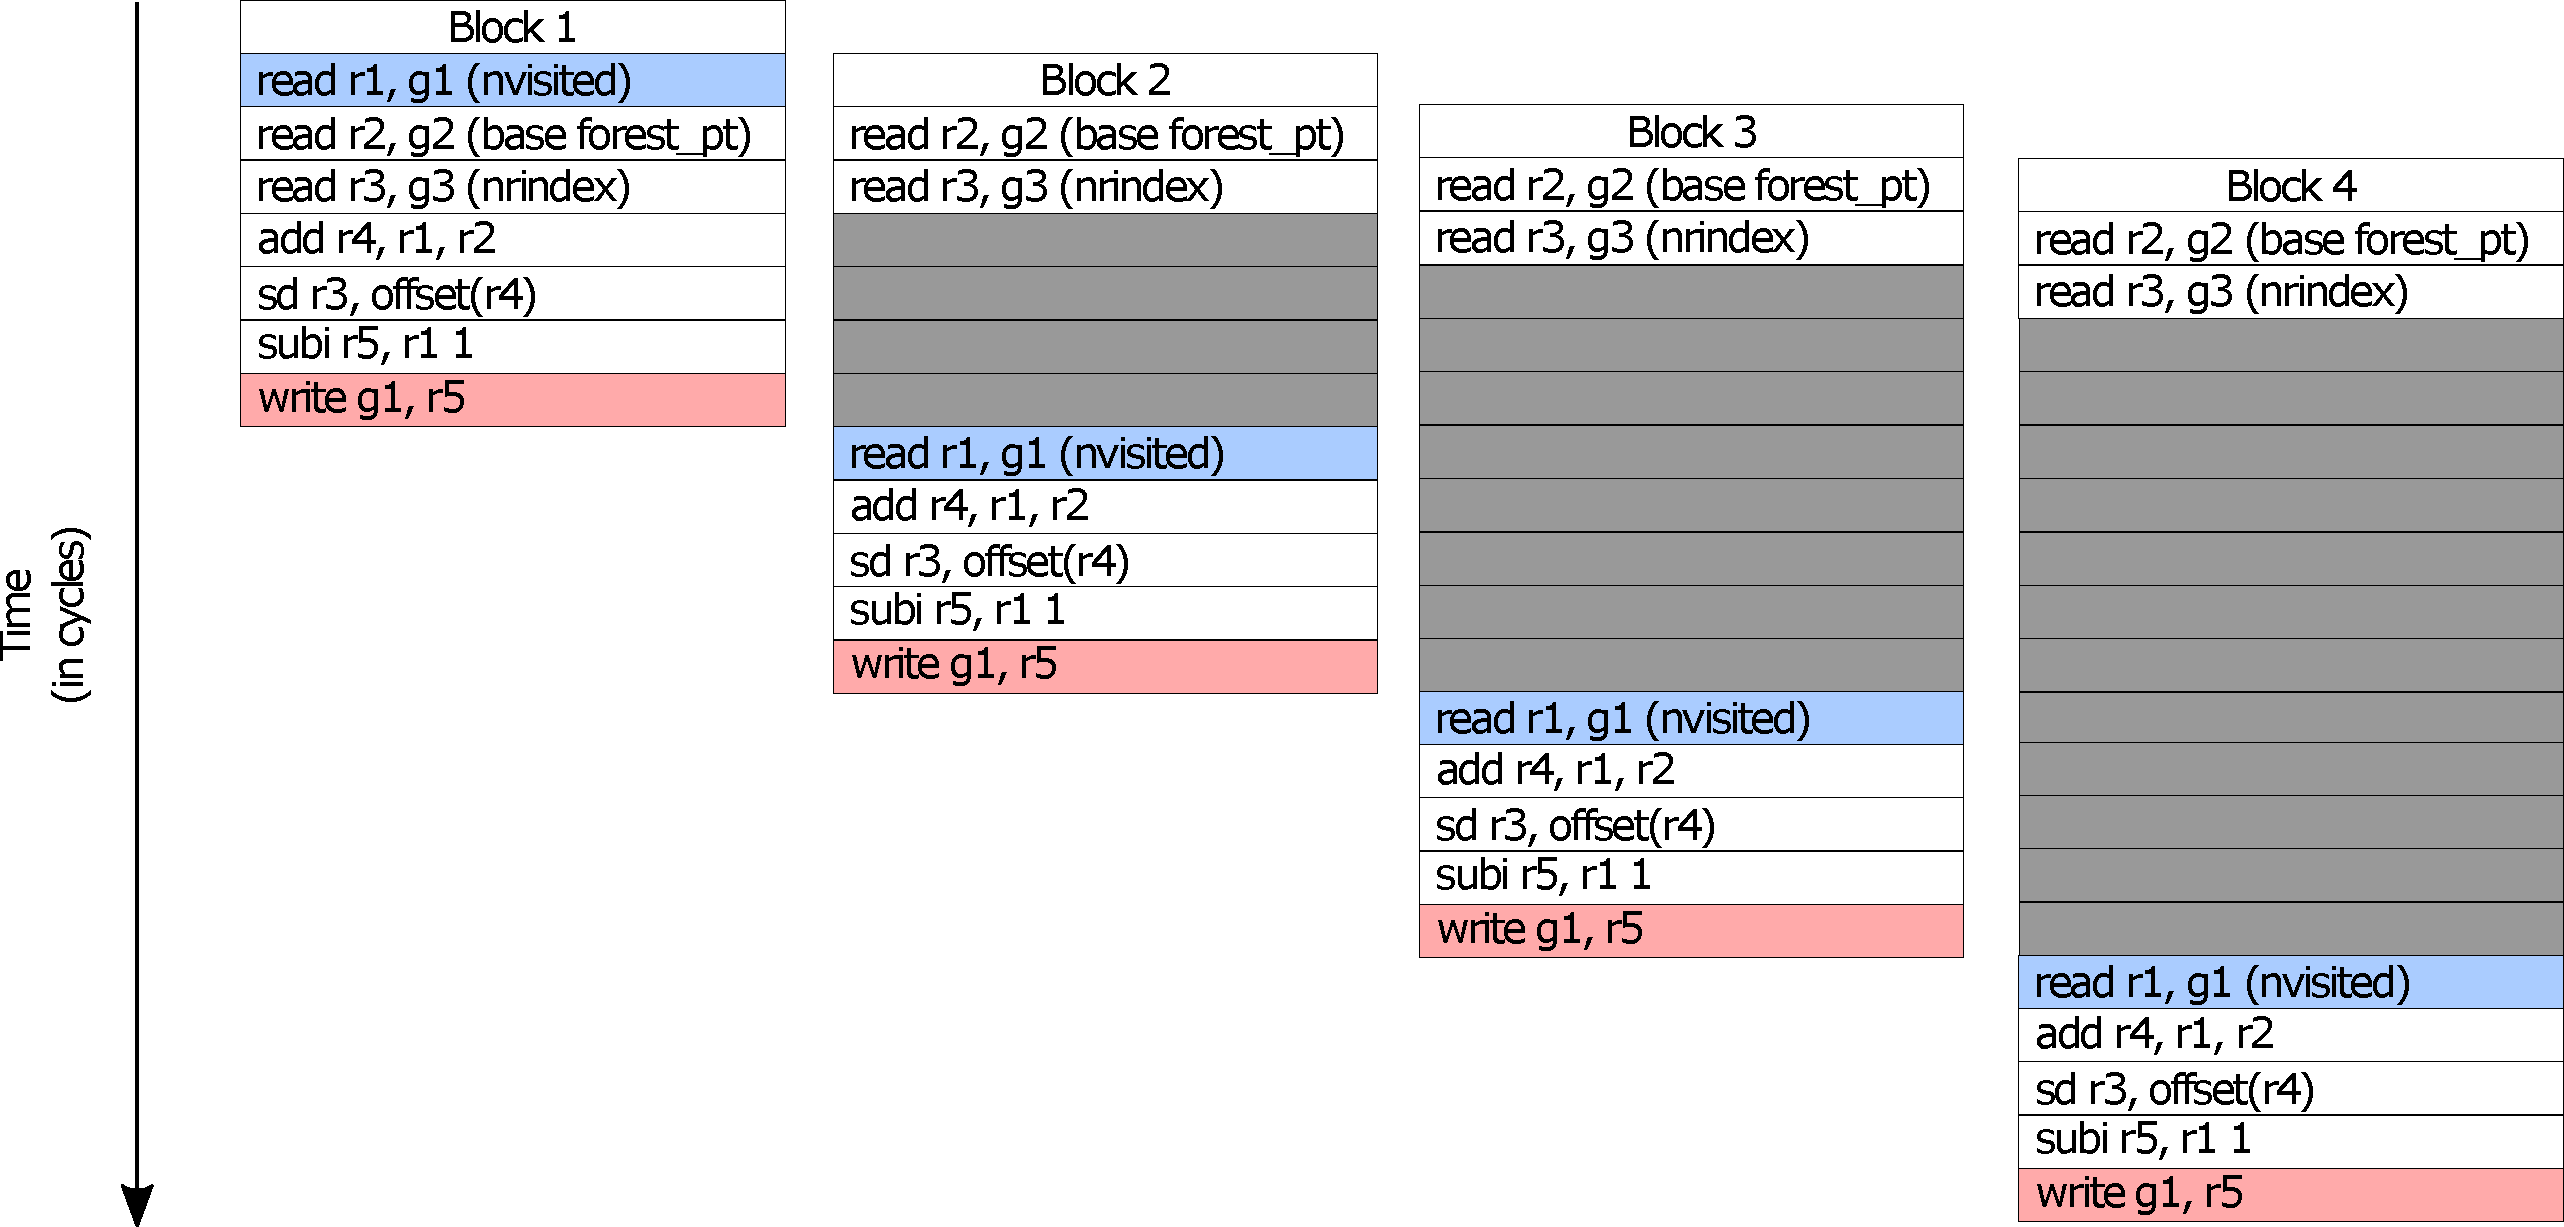
\includegraphics[width=1\textwidth]{chapter3/graphics/mser_ex.pdf}
		\captionof{figure}{Example of how data-dependencies cause delays when executing four blocks in parallel. The numbers represent part of the loop body in Listing~\ref{lst:mser_snipet}.}
    \label{fig:mser_nvsited}
	\vspace{1em}
\end{figure}

%If multiple blocks representing Listing~\ref{lst:mser_snipet} are in flight, the youngest block reading the value of \textit{nvisited} will have to wait for the previous block to execute the write.
%In such a case, a data dependency arises when executing multiple blocks in parallel if a write to a register which has to be read by multiple blocks is pending.
%This can be especially problematic when large core compositions are used, as up to 64 blocks can potentially be in flight at any moment.

To illustrate the data-dependency problem, Figure~\ref{fig:mser_nvsited} shows a simplified view of four blocks representing the body of the loop in Listing~\ref{lst:mser_snipet} being executed in parallel.
Each block starts executing a cycle after its parent; the instructions highlighted in colour represent the register causing the data-dependency; blue represents the register being read, and red represents the register being written to.
The grey slots represent cycles where the block cannot execute any instructions.
Assuming each instruction takes a single cycle to execute, 22 cycles are needed to execute all four blocks in parallel, compared to 28 cycles if they were to be executed sequentially.
If the data dependencies are not resolved quickly enough, then this causes blocks to execute in a serial fashion, which reduces any benefit from using the composition.

\begin{figure}[t]
    \centering
    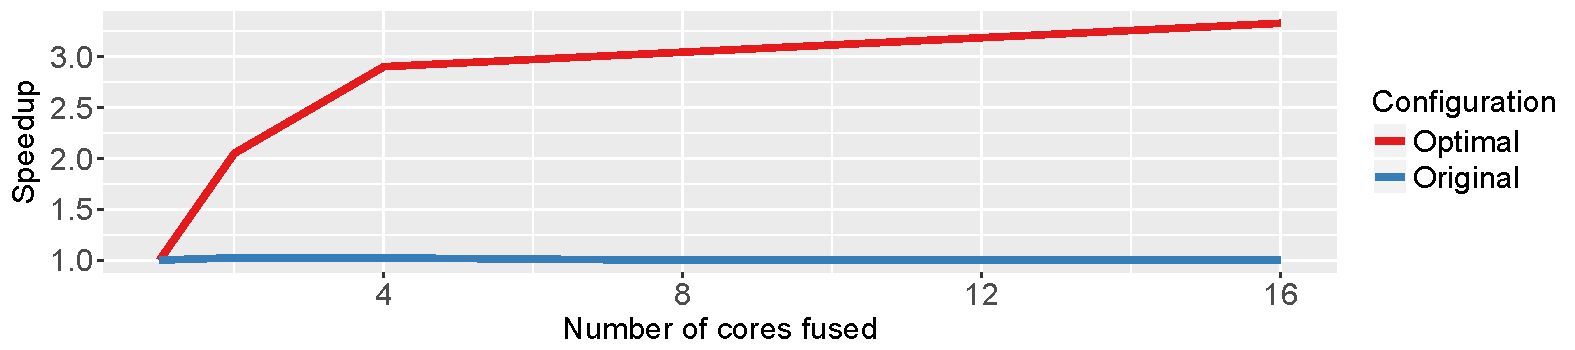
\includegraphics[width=1\textwidth]{chapter3/graphics/mser_motiv_reg2.pdf}
    \caption{Speedup of executing \bm{MSER} using the new fetching mechanism, with perfect value prediction and perfect branch prediction. Baseline is a single core with original branch prediction accuracy. Higher is better.}
    \label{fig:motivation_reg}
	\vspace{1em}
\end{figure}


If cores do not have to wait on data dependencies, this can increase efficiency of core compositions, as they can execute their blocks independently.
Figure~\ref{fig:motivation_reg} shows how an optimal configuration of the processor, one that can fetch blocks in parallel, has perfect branch prediction and can immediately resolve data dependencies can improve performance on \bm{MSER}.
The speedup is obtained by comparing the execution time of core compositions to a normal single core, without perfect branch prediction.
The figure also shows the performance of a ``normal" core composition configuration that has no perfect branch prediction, serialised block fetches and cannot resolve data dependencies immediately.
As shown in the Figure~\ref{fig:motivation_reg}, a 16 core composition can now get a speedup of up to 3x, compared to the 2x when using only perfect branch prediction and the OF scheme.
%This is due to the fact that register dependencies are no longer serialising some of the computation between blocks, and thus blocks can be executed in parallel.

Serialised execution due to data dependencies is a common problem for superscalar processors~\cite{peraisVTAGE2014}.
One solution to the problem is adding a value predictor to the processor, which is able to predict the value of a register.
This allows instructions to execute with speculative data, and thus increase ILP and reduce the impact of data-dependencies.
Section~\ref{chp3:sec:val} covers the implementation of a value predictor for an EDGE processor which is used throughout this chapter.



%\subsection{Putting it all together}

%The previous 3 sections demonstrate that with modifications of the hardware, a previous benchmarks that showed very little performance gains with core composition can now see a performance increase of up to 1.90x on a 4 core composition.
%This demonstrates that the hardware used for core composition can be improved in order to tackle difficult applications.
%Whilst the previous three sections accumulated hardware modifications to obtain the 1.90x speedup, it is important to show how all these changes must be included in the processor in order to obtain the best results.

%\begin{figure}[t]
%    \centering
%    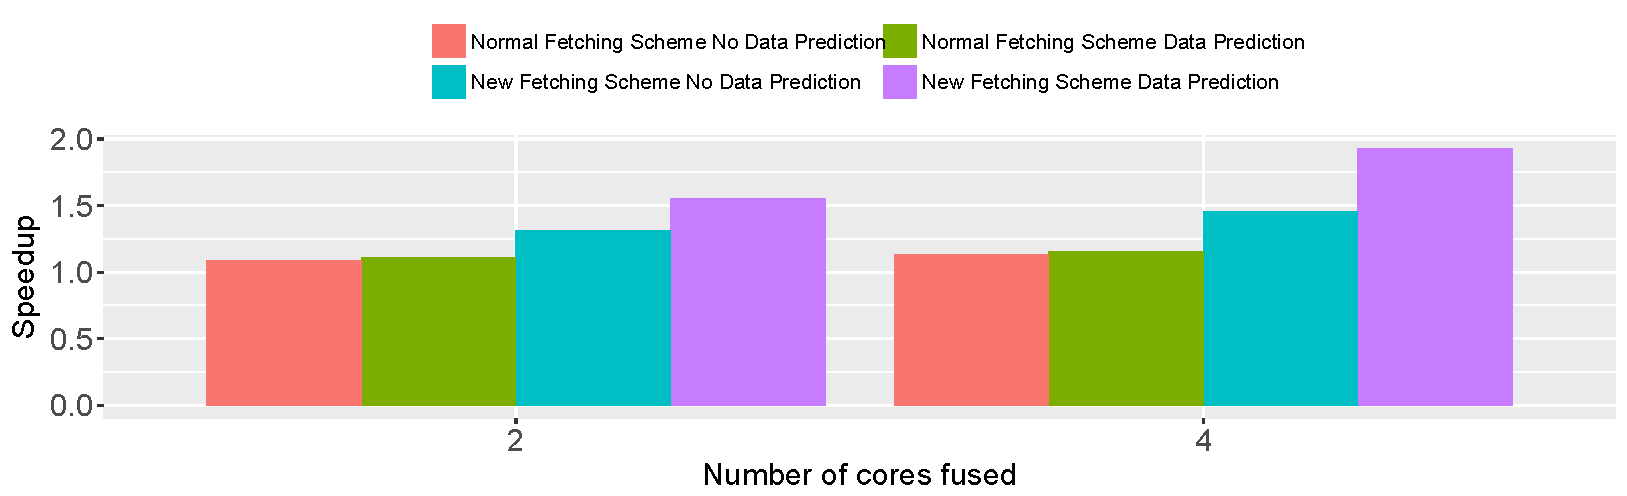
\includegraphics[width=1\textwidth]{chapter3/graphics/mser_final_motiv.pdf}
%    \caption{Speedup obtained when executing the MSER benchmark on 2 and 4 core composition with the new fetching scheme. Higher is better.}
%    \label{fig:motivation_final}%
%	\vspace{1em}
%\end{figure}

%Figure~\ref{fig:motivation_final} shows how the performance of \bm{MSER} is improved on when adding either the new fetching scheme, the value predictor, or both.
%The performance is compared to a single core with or without value prediction; all the experiments use a perfect branch predictor.
%Overall, the figure reveals that the current fetching scheme -- even with perfect value prediction and perfect branch prediction -- cannot obtain any significant performance improvements.
%This is due to the fact that the core compositions are limited by the serialisation of block fetches.
%Adding value prediction does not improve performance greatly because of the fact that it reduces the execution time of blocks, which once again increases the difficulty of populating cores with blocks.

%On the other hand, the figure also highlights that modifying the fetching scheme does not suffice in order to get the fastest execution times.
%%This is due to the fact that if cores are able to fetch blocks at a much faster rate, they will then be limited by potential register dependencies.
%Therefore, it is important to consider multiple modifications to the hardware in order to get the best performance.

%Finally, it is important to remember that these results are currently only made possible through the use of perfect branch prediction.
%Executing \bm{MSER} without perfect branch prediction leads to an average accuracy of 86\%, which is not enough to ensure that core composition can be efficiently used.
%This motivates exploring the potential performance of core composition through the use of a perfect branch predictor.
